\chapter{Stand der Technik}

%%%%%%%%%%%%%%%%%%% Mechanik

\section{Kühlung} 

Bei dem Vorgang der Kühlung oder Abkühlung, wird einem System Wärme, oder thermische Energie entzogen. (Deshalb auch Entwärmung genannt)
Unter Kühlung versteht man die Übertragung von Wärme einer technischen Komponente, an die Umwelt. Dieses Phänomen wird oft beabsichtigt hervorgerufen, um bestimmte temperaturabhängige Eigenschaften erreichen und erhalten, aber auch Systeme vor Überhitzung schützen zu können. 
Durch Isolierungen, wie beispielsweise bei Häusern, kann unerwünschter Wärmeentzug zu einem gewissen Teil verhindert werden.

\subsection{Thermodynamische Grundlagen}

Der Entzug von Wärme geht bei Feststoffen und Flüssigkeiten durch Wärmeübertragung entsprechend einem Temperaturgradienten vonstatten. Die wesentlichen Prozesse sind dabei Wärmeleitung und Wärmestrahlung, eingeschränkt auch die Konvektion. Da all diese Prozesse spontan ablaufen und folglich entsprechend den Grundgesetzen der Thermodynamik einen Temperaturausgleich zur Folge haben, kann eine künstlich erwünschte Kühlung eines Gegenstandes gegen einen Temperaturgradienten nur unter hohem Energieaufwand erfolgen. 

Insgesamt wird dies jedoch immer mit einer Erhöhung der Gesamtentropie und damit im Regelfall einer Umwandlung Energieformen höherer Ordnung in thermische Energie resultieren. Eine Kühlung im Sinne einer Reduzierung der thermischen Energie eines abgeschlossenen Systems ist daher nicht möglich, was sich in der Praxis zum Beispiel darin äußert, dass auch Kühlschränke letztlich die Temperatur (der Umgebung) erhöhen und nicht senken, wenn dies auch lokal der Fall sein mag.

Die entscheidenden Einflussfaktoren sind dabei durch Wärmeleitkoeffizient, Wärmeübergangskoeffizient und Wärmekapazität gegeben. Bei Flüssigkeiten spielt die Wärmeleitung und Wärmestrahlung ebenfalls eine Rolle, hinzu kommt jedoch die Konvektion als wesentlicher Prozess des Temperaturausgleichs. Dieser dominiert hingegen bei Gasen, wobei diese allgemein nur sehr schlecht über Prozesse der Wärmeleitung abkühlen. Sie unterliegen jedoch verschiedenen Gasgesetzen, wodurch vor allem der adiabatischen Abkühlung und dem Joule-Thomson-Effekt eine große Rolle zukommt. 

\subsection{Technische Anwendung}

Kühlsysteme können nach dem verwendeten Wärmeträgermedium unterteilt werden. Die geläufigsten Arten der Kühlung sind:

\begin{itemize}
	\item Wasserkühlung und
	\item Luftkühlung.
	\item Ölkühlung z.  B. im Automotor und in Hydrauliksystemen (hydraulischen Antrieben) 
	\item Natriumkühlung in Kernkraftwerken
	\item Kühlung durch Peltier-Elemente Kühlung von Prozessoren
\end{itemize}

\subsection{Funktionsweise}

Eine Kühlung basiert meist auf der Übertragung der Wärme (Wärmeleitung) vom zu kühlendem Körper zum Kühlstoff (Gas oder Flüssigkeit) und deren Abtransport (Wärmeströmung).
Bei manchen Anwendungen mit engen Platzverhältnissen (innerhalb eines Computers oder HiFi-Verstärkers) werden zum Abtransport Heatpipes verwendet.
Bei den meisten Motoren wird eine spezielle Kühlflüssigkeit eingesetzt.

\subsection{Einsatzgebiete}

Kühlungen werden in fast allen technischen Geräten, die sich erwärmen, eingesetzt. Zumeist wird jedoch eine passive Kühlung, das heißt die Abgabe der Wärme über Kühlkörper an die umgebende Luft, genutzt.
Das bekannteste Beispiel ist der Kühlschrank zur Konservierung von Lebensmitteln. In Kfz wird meist eine Wasserkühlung benutzt, in Computern kommen überwiegend Luftkühlungen zum Einsatz. Ein weiteres großes Einsatzgebiet ist zum Beispiel die Klimaanlage.

\subsection{Beispiele}

\begin{itemize}
	\item Kühlsysteme von Kraftwerken und chemischen Prozessen
	\item Kühlung in der Klimatechnik
	\item Öl- und Ladeluftkühler im Turbodiesel-Motor
	\item Abgaskühlung in AGR-Systemen (zur Emissionsreduzierung (NOx))
	\item Wasserkühlung eines Automotors
	\item Luftkühlung eines Prozessors
\end{itemize}

%Quelle: https://www.chemie.de/lexikon/K%C3%BChlung.html 09:29 Uhr 17.03.2021
%Dieser Artikel basiert auf dem Artikel Kühlung aus der freien Enzyklopädie Wikipedia und steht unter der GNU-Lizenz für freie Dokumentation. In der Wikipedia ist eine Liste der Autoren verfügbar.

Zu Kühlung siehe auch \cite{Kuehlung1,Kuehlung2}

\newpage

\subsection{Wasserkühlung} 

Bei einer Wasserkühlung (Flüssigkeitskühlung), wird Wasser als primäres Kühlmittel verwendet wird. Die Wasserkühlung kann sehr vielseitig eingesetzt werden. Wasser wird als Kühlung in Elektro- wie auch in Verbrennungsmotoren, Hochöfen, Stromrichtern, Kraftwerken, Computern und noch vielen weiteren Anwendungen verwendet.   

\subsubsection{Wasserkühlung bei elektronischen Geräten}

Seit 1930 werden die röhrenbestückten Endstufen von Hochleistungssendern mit Wasser gekühlt. Da hierbei hohe elektrische Spannungen zum Einsatz kommen, kann nur destilliertes deionisiertes Wasser zum Einsatz kommen. Dieses gibt in einem Wärmeübertrager seine Wärme an einem zweiten Kreislauf ab, in dem das Wasser keinen besonderen Reinheitsanforderungen genügen muss, da es mit keinen spannungsführenden Komponenten in Kontakt kommt.

Bei Hochleistungsröhren wird die Siedekondensationskühlung angewandt. Bei dieser Technik sind Dampferzeugung und Kondensation räumlich nicht voneinander getrennt. Das Kühlmittel durchfließt den Kühlkanal, der mit zur Anodeninnenseite hin orientierten Nuten ausgestattet ist. Der in diesen Nuten entstehende Dampf gerät in den Hauptkühlkanal, wo er verwirbelt wird und wieder kondensiert. Da sich dieser Vorgang bei Temperaturen von über 100 °C abspielt, und den Aggregatzustand flüssig zu gasförmig nutzt, können mit diesem Kühlverfahren auf Grund der dafür notwendigen Verdampfungswärme auch bei relativ kleinen Röhren große Wärmemengen abgeführt werden.
Moderne, halbleiterbestückte Sender haben keine Wasserkühlung mehr.
Wasserkühlung wird auch in der Leistungselektronik angewandt. Zum Beispiel für Stromrichter in Anlagen der Hochspannungs-Gleichstrom-Übertragung oder für Traktionsstromrichter in Schienenfahrzeugen.


\subsubsection{Wasserkühlung in Personal Computern}

Wasserkühlungen werden auch in modernen PC-Systemen zur leisen und effektiven Kühlung einzelner Komponenten eingesetzt. Dabei wird am häufigsten der Hauptprozessor gekühlt. Weitere Komponenten, die in den Kühlkreislauf eingebunden werden können, sind Grafikkarten, Hauptplatinen­chipsätze, Festplatten, Netzteile, Spannungswandler und auch RAM-Bausteine.
Wasserkühlungen für PCs sind in PC-Moddingkreisen sehr verbreitet. Mittlerweile ist ein großer Markt um Wasserkühlungen entstanden.
Die Vorteile einer Wasserkühlung sind zum einen die effektive Kühlung der Hardware mit für Modder und Overclocker wichtigem Übertaktungsspielraum der CPU durch verbesserte Wärmeabfuhr. Zum anderen arbeitet die Kühlung fast lautlos, da auf dem Radiator (Wärmeübertrager) große, langsam drehende Lüfter eingesetzt oder auch passive Radiatoren ohne Lüfter verwendet werden können. Außerdem erhöht sich in der Regel die Zuverlässigkeit und Lebensdauer der mit Wasser gekühlten Komponenten. Je nach verwendeter Pumpe kann die Wasserkühlung eine der stromsparendsten Kühlungsmethoden sein.
Nachteilig ist der erheblich größere Installationsaufwand, die vergleichsweise hohen Kosten und der Wartungsbedarf. Häufig führt der Verzicht auf den Einsatz von Gehäuselüftern dazu, dass einzelne Komponenten überhitzen, die nicht in den Kühlkreislauf einbezogen werden können. Je nach Anzahl der verbauten Komponenten kann ein grösserer Platzbedarf im Gehäuse erforderlich sein.
Reines destilliertes Wasser besitzt verglichen mit allen anderen natürlichen Stoffen, die bei Zimmertemperatur flüssig sind, den höchsten Wärmeleitkoeffizienten und ist daher erste Wahl beim Bau einer Flüssigkühlung.

Zu Wasserkühlung siehe auch \cite{Wasserkuehlung}
%Quelle https://www.chemie.de/lexikon/Wasserk%C3%BChlung.html 09:50 Uhr 17.03.2021
%Dieser Artikel basiert auf dem Artikel Wasserkühlung aus der freien Enzyklopädie Wikipedia und steht unter der GNU-Lizenz für freie Dokumentation. In der Wikipedia ist eine Liste der Autoren verfügbar.

\newpage

\subsection{Luftkühlung} 

Durch Luftkühlung wird die Oberfläche von wärmeerzeugenden Objekten wie elektronischen Bauelementen der Leistungselektronik, Verbrennungsmotoren und Klimaanlagen durch daran vorbei strömende Luft gekühlt.
Die zur Luftkühlung notwendige Luftbewegung kann entweder durch Konvektion, Gebläse oder bei Fahrzeugen durch den Fahrtwind bewirkt werden. Das zu kühlende Objekt steht frei oder wird kanalisiert umflossen. Häufig ist das zu kühlende Objekt auch mit Kühlrippen oder einem Kühlkörper als Wärmeübertrager versehen, die durch eine größere Oberfläche einen größeren Wärmeabfluss ermöglichen.

\subsubsection{Luftkühlung bei Personalcomputern}

Im Verhältnis zur Baugröße geht - insbesondere bei Prozessoren ab der Klasse Intel 486/66 - mit der kommerziell wirtschaftlich zur Verfügung stehenden Technologie eine große Wärmeentwicklung einher. Leistungsstarke Mikrochips, wie sie in aktuellen PCs verwendet werden, erzeugen erhebliche Verlustwärme, die überwiegend durch eine Luftkühlung abgeführt wird. Zweck ist, eine thermische Überlastung der Chips zu verhindern.

Da die gesamte Aufnahmeleistung in Wärme umgesetzt wird, wurde zunächst die Betriebsspannungen der wärmeerzeugenden Komponenten reduziert. Ferner werden in aktuellen Prozessoren Teile des Rechenwerkes bei Nichtgebrauch in der Taktfrequenz reduziert oder ganz abgeschaltet. Trotzdem reichte die natürliche Wärmeabfuhr durch Strahlung und Konvektion nicht mehr aus, so dass die thermisch wirksamen Oberflächen erst durch den Einsatz von Kühlkörpern gekühlt wurden und dann - weil immer noch nicht ausreichend - die mögliche Wärmeabfuhr durch Einsatz von elektrisch betriebenen Ventilatoren vergrößert wurde (vgl. Prozessorkühler). 

Das am stärksten gekühlte System in PCs ist die CPU, doch auch das Netzteil und seit einiger Zeit auch die Prozessoren von Grafikkarten werden luftgekühlt. Alternativ dazu kann man auch in PCs eine Wasserkühlung einbauen.

Weitere Anwendungen:
\begin{itemize}
	\item HiFi-Verstärker 
	\item Spanen an hygroskopischen(Feuchtigkeitziehenden) Kunststoff
\end{itemize}

Zu Luftkühlung siehe auch \cite{Luftkuehlung1,Luftkuehlung2}

%Quelle: https://www.chemie.de/lexikon/Luftk%C3%BChlung.html 10:56 Uhr17.03.2021#
%Dieser Artikel basiert auf dem Artikel Luftkühlung aus der freien Enzyklopädie Wikipedia und steht unter der GNU-Lizenz für freie Dokumentation. In der Wikipedia ist eine Liste der Autoren verfügbar.

\subsection{Ölkühlung}

Unter Ölkühlung versteht man eine Kühlung mit Öl. Die Ölkühlung wird hauptsächlich für leistungselektrische Geräte, wie Transformatoren angewandt, wobei das Öl auch die Funktion der Isolation übernimmt. Bei der Ölkühlung befindet sich das wärmeentwickelnde Element in einem Ölbad, welches mit einem Ausdehnungsgefäß ausgestattet ist, um Volumenschwankungen des Öls auszugleichen.

%Quelle: https://www.chemie.de/lexikon/%C3%96lk%C3%BChlung.html 10:59 Uhr 17.03.2021
%Dieser Artikel basiert auf dem Artikel Ölkühlung aus der freien Enzyklopädie Wikipedia und steht unter der GNU-Lizenz für freie Dokumentation. In der Wikipedia ist eine Liste der Autoren verfügbar.

\newpage

\subsection{Aktive Kühlung} 

Bei aktiver Kühlung wird die zu kühlende Komponente mit Hilfe eines Lüfters oder einer Pumpe gekühlt.
\subsubsection{Aufbau}

Im Regelfall besteht eine aktive Kühlung aus folgenden Komponenten:
Kühlmittel kann aus Luft, Wasser oder einer speziellen Kühlflüssigkeit bestehen, welche meist noch für eine Schmierung der Bauteile sorgt.
Lüfter oder Pumpe, welcher einen Kühlmittelstrom erzeugt der den Wärmeübertrager Radiator durchströmt und das Kühlmedium auf seine Ausgangstemperatur herunterkühlt, oder aber durch den Luftstrom das zu kühlende Bauteil direkt kühlt.

Funktionsprinzip: Flüssigkühlung
Das Kühlmedium (Wasser, Kühlmittel) wird mit Hilfe einer Pumpe durch diverse Leitungen an das zu kühlende Bauteil befördert. Dort umströmt es entweder das Bauteil direkt oder fließt durch einen speziellen Aufsatz am zu kühlenden Bauteil (z.B. Prozessor in einer PC-Wasserkühlung).
Hierbei nimmt das Kühlmittel die Wärme des Bauteils auf und transportiert sie beim Weiterfließen ab.
Das Kühlmittel fließt anschließen, (bei nur einer zu kühlenden Komponente), durch den Radiator welcher aktiv mit Lüfter, oder passiv ohne Lüfter, dafür aber größer ausgelegt sein kann.

Durch den Radiator kann das Kühlmedium die Wärme an die Umgebung abgeben. Ein Temperaturgefälle ist dazu immer notwendig; je größer das Temperaturgefälle, desto größer die Wärmemenge, die je Zeiteinheit und Fläche übertragen werden kann.
Funktionsprinizp Luftkühlung

Zu Aktive Kühlung siehe auch \cite{AktiveKuehlung}

%Quelle: https://www.chemie.de/lexikon/Aktive_K%C3%BChlung.html 11:03 Uhr 17.03.2021
%Dieser Artikel basiert auf dem Artikel Passive_Kühlung aus der freien Enzyklopädie Wikipedia und steht unter der GNU-Lizenz für freie Dokumentation. In der Wikipedia ist eine Liste der Autoren verfügbar.

\newpage
\section{Akkusysteme}
Verschiedene Speicher für elektrische Energie, die auf einer elektrochemischen Basis basieren, nennt man Batterien oder auch Akkumulatoren. Elektrochemische Speicher haben in den vergangenen Jahren immer mehr an Bedeutung gewonnen und werden auch in Zukunft immer öfter Gebrauch finden. Möglich wurde unsere heutige elektronische Mobilität erst mit der Erfindung der galvanischen Zelle. Seit dieser Erfindung,die mit Hilfe eines Stromkreises chemische Energie in elektrische Energie umzuwandeln, hat sich über die jahrzehntelange Weiterentwicklung der Batterie einiges getan. Die Einsatzmöglichkeiten von Akkumulatoren sind extrem vielfältig. Kleine Lithium-Ionen Akkus werden zum Beispiel als Knopfzellen in Smartphones verwendet. Jedoch können sie auch bis hin zu großen stationären Energiespeichern für erneuerbare Energien benutzt werden. Wie bereits vorher erwähnt, sind elektrische Energiespeicher ein wichtiger Bestandteil für den Erfolg der Elektromobilität geworden. Es gibt unzählig viele verschiedene Arten von Batterien, die sich im chemischen Aufbau, ihrer Form und natürlich in ihren Einsatzmöglichkeiten unterscheiden. Durch die äußerst besonderen chemischen Eigenschaften und die vielseitigen Anwendungsbereiche, hat sich der Lithium-Ionen Akku durchgesetzt.
\newpage

\section{Batteriearten}

\subsection{Bleiakkumulator}
Die ersten Versuche, einen auf Blei basierenden Akkumulator zu entwickeln, wurden am Anfang des 19. Jahrhunderts durchgeführt. Industriell wurde der Bleiakku interessant, als Forscher und Chemiker zusammen 1880 ein Verfahren entwickelten, bei dem der Bleiakkumulator bereits nach wenigen Ladezyklen, eine hohe Kapazität erreichte. Der erste technisch einsetzbare Bleiakkumulator wurde 1886 von Henri Tudor entwickelt. Dieser besitzt eine Zellspannung von ungefähr 2V (abhängig vom Ladezustand), was eine durchaus große Spannung für sogenannte "wässrige Syteme"  ist. Der Ausdruck "wässrige Systeme"  leitet sich von dem Elektrolyt ab. Bei Bleiakkumulatoren wird wässrige Schwefelsäure als Elektrolyt verwendet. Im entladenen Zusatnd bestehen beide Pole aus Blei(II)-sulfat (PbSO4). Weiters besteht die Kathode aus Blei und die Anode aus Bleioxid. Bleiakkumulatoren sollten keinesfalls tiefenentladen werden, da dies zu Schäden führt und den Akku unbrauchbar macht. Ein extrem großer Nachteil ist das Gewicht, da nur 30 bis 40Wh/kg erreicht werden können.
Diese Art von Akku zeichnet sich durch das kurzzeitige Zulassen hoher Ströme aus die zum Beispiel für Fahrzeug -bzw. Starterbatterien notwendig sind. Unter anderem sind 50 Prozent des Batteriemarkets von Bleiakkumulatoren belegt. Wie vorher bereits erwähnt werden diese oftmals in Autos, LKWs oder auch Motorräder verbaut.

\subsection{Nickel-Metallhybrid Akkumulatoren}
Die technischen Grundlagen des Nickel-Metallhybrid Akkumulator wurden von Stanford R. Ovshinsky und Masahiko Oshitani ab 1962 bis 1982 zur marktreifen Zelle entwickelt. Seit dem Jahr 2006 sind spezielle NiMH-Akkumulatoren auf dem Markt, die sich gegenüber herkömmlichen NiMH-Akkus durch eine deutlich reduzierte Selbstentladung auszeichnen. Die positive Elektrode eines Nickel-Metallhybrid Akkumulators(NiMH) besteht aus Nickel(II)-hydroxid wogegen sich die negative Elektrode aus einem Metallhybrid zusammensetzt. Als Elektorlyt verwendet dieser Akkumulator eine Wasserstoffspeicherlegierung aus Nickel und seltenen Erden. NiMH-Akkus erreichen bis zu 80Wh/kg. Sie sind vielfach in den üblichen Bauformen von Standardbatterien verbreitet und liefern pro Zelle eine Spannung von 1,2V. Oftmals werden sie als wiederaufladbare Alternative der gängigen Alkalibatterien in haushaltsüblichen Geräten eingesetzt. Ein großer Vorteil gegenüber den Nickel-Cadmium Batterien ist es, das der NiMH Akku nicht aus giftigen Cadmium besteht und er außerdem eine höher Energiedichte aufweist.
Der Anwendungsbereich von NiMH Akkumalatoren ist sehr vielfältig. Vorzugsweise kommen sie wie NiCd Akkus überall dort zur Anwendung, wo ein hoher Energiebedarf besteht und hohe Batteriekosten vermeiden werden sollten. Tyische Anwendungsbereich sind zum Beispiel Foto- Videogeräte, Elektroautos, Elektrowerkzeuge und noch viele mehr. NiMH Akkus werden außerdem oft als Energiespeicher für Notbeleutungsanlagen verwendet.
\newpage
\subsection{Nickel-Cadmium Akkumulatoren}
1899 wurde der Nickel-Cadmium Akku von dem Schweden W. Jungner entwickelt. NiCd Akkus zeichnen sich dadurch aus, dass sie einen eingebauten Ent- und Überladeschutz integriert haben. Das hat zur Folge, dass man keine aufwendige elektronische Beschaltung durchführen muss. Als Material für die Kathode dieses Akkus verwendet man Nickeloxidhydroxid. Die Anode dagegen besteht aus dem giftigen Material Cadmium, welches jedoch eine äußerst hohe spezifische Ladung (478Ah/kg) besitzt. Bei Nickel-Cadmium Akkumulatoren besteht das Elektorlyt aus Kalilauge. Die typische Nennspannung ist exakt die selbe wie bei NiMH Akkus, 1,2V. Aus dieser Zellenspannung ergibt sich eine spezifische Energie von ungefähr 60Wh/kg. Eine Eigenschaft die man bei anderen Technologien nur selten antrifft ist das hervorragende Tieftemperaturverhalten von NiCd Akkus. Selbst bei einer Temperatur von -40°C ist eine Inbetriebnahme noch möglich. Im Jahr 2004 wurde jedoch die Verwendung von Nickel-Cadmium Akkus wegen dem giftigen Material auf medizinische und sicherheitrelevante Bereiche begrenzt. Diese Akkumulatoren sind in 2 verschiedenen Bauformen verfügbar, die sich durch die unterschiedlichen Anwendungsbereiche unterscheiden. Die offene Bauweise wird meist für Starterbatterien für Verbrennungsmotoren und Traktionsbatterien für Elektrofahrzeuge verwendet. Bei der anderen Bauweise, werden die Zellen gasdicht verschlossen. Oftmals werden sich für zentrale Stromversorgungssysteme für Notbeleuchtung verwendet.
\newpage

\subsection{Lithium-Ionen Batterie}
\subsubsection{Geschichte}
Schon bereits in dem Jahr 1970 wurde von Jürgen Otto Besenhard und anderen das grundlegende Funktionsprinzip der Alkalimetallionen-Interkalation in Kohlenstoff-Elektroden sowie auch in oxidischen Elektroden erforscht und veröffentlicht. Ebenfalls wurde dabei die Anwendung in Lithium Batterien untersucht auch wenn zu der Zeit die praktische Anwendbarkeit als Elektroden für Lithium Batterien noch nicht erkannt wurde. Der erste auf dem Markt erhältliche Lithium-Ionen Akkumulator wurde von Sony im Jahr 1991 angeboten. Dieser Lithium-Cobaltdioxid Akku wurde in einer Videokamera verbaut. Die Batterie, die eine Spannung von 7,2V aufweiste, bestand aus zwei seriell verschalteten Zellen und weiste etwa eine Kapazität von 1200mAh auf. Sogar bis heute wird diese Bauform von Akkumulatoren mit Kapazitäten
bis zu 6900mAh angeboten und in äußerst vielen Geräten eingesetzt. Drei Physiker bzw. Chemiker (Whittingham, Goodenough und Yoshino) erhielten 2019 sogar den Nobelpreis für Chemie, für die Entwicklung der Lithium-Ionen Batterie.
Forscher einer Universität fanden im Jahr 2020 heraus, dass durch die Zugabe von dem Element Kalium die Lithium Akkumulatoren langlebiger und sicherer werden. Außderdem verhindert das Kalium in dem Akku unerwünschte chemische Nebenreaktionen.
\subsubsection{Allgemeines}
Es gibt zahlreiche verschiedene Bauformen von Lithium-Ionen Akkumulatoren. Diese Batterien unterscheiden sich nicht nur in ihrer Größe und der Bauform, sondern auch in der chemischen Zusammensetzung ihrer Komponenten und haben unter anderem auch verschiedene Spannungsbereiche. Kenndaten wie Zellenspannung, Lade- und Entladeschlussspannung, Temperaturempfindlichkeit und der maximal zulässige Lade- oder Entladestrom variieren bauartbedingt und sind wesentlich vom eingesetzten Elektrodenmaterial und den Elektorlyten abhängig. Eine Eigenschaft die alle Lithium-Ionen Akkumulatoren gemeinsamen haben ist, dass sie gasdicht versiegelt sein müssen und außerdem lageunabhängig betrieben werden können. Die spezifische Energiedichte liegt ungefähr in der Größenordnung von 150Wh/kg und weist eine Energiedichte von 400Wh/l auf. Durch diese Eigenschaften findet diese Art von Batterie besonderen Einsatz in der mobilen Branche als elektrischer Energiespeicher. Ein weiteres wichtiges Merkmal aller Lithium-Ionen Akkumulatoren ist, dass sie Überladungen nicht verkraften können. Wenn man mehrere Zellen zum Beispiel in Reihe schaltet, um eine höhere elektrische Spannung zu erzielen, müssen zum Ausgleichen der Toleranzen in der Kapazität zwischen den Zellen meistens zusätzlich ein Batteriemanagementsystem (BMS) und ein Balancer vorgesehen werden.  
\newpage

\subsubsection{Prinzip der Lithium-Ionen Batterie}
Ein Lithium-Ionen Akkumulator erzeugt durch die Verschiebung von Lithium-Ionen eine elektromotorische Kraft.
Beim Ladevorgang wandern positiv geladene Lithium-Ionen durch einen Elektrolyten hindurch von der positiven Elektrode zur negativen, während der Ladestrom die Elektronen über den äußeren Stromkreis liefert. Eine negative Elektrode aus Lithium-Metall ist elektrochemisch optimal, für einen Akku aber ungeeignet. Da sich die Elektrode beim Entladevorgang genauso wie bei einer Lithium-Batterie auflöst, besteht beim Ladevorgang keine Möglichkeit mehr, ihre Geometrie zu rekonstruieren.

\textbf{Aufbau:}

Die negative Elektrode eines gänigen Lithium-Ionen Akkus besteht meist aus Graphit. Die positive Elektrode hingegen enthält meist Lithium-Metalloxide in Schichtstruktur wie Lithiumcobaltoxid (LiCoO2). Der Lithium-Ionen Akkumulator muss wasserdicht sein, da es sont zu einer Nebenreaktion zwischen dem Wasser (H2O) mit dem Leitsalz (LiPF6) zu Flusssäure (HF) reagieren kann. Das am häufigsten verwendete Elektrolyt in Lithium-Ionen Akkumulatoren besteht aus einer Mischung zwischen wasserfreien Lösungsmitteln (Ethylencarbonat, Propylencarbonat) mit Alkylcarbonaten/Äthern (Dimethylcarbonat, Diethylcarbonat) und natürlich mit Lithiumsalzen.

Beim Aufladen der Lithium-Ionen Akkus, d.h. anlegen einer äußeren Potenzials, fließen Lithium-Ionen zwischen die Graphitebenen (nC). Zusammen mit dem Kohlenstoff bilden diese Ionen eine Interkalationsverbindung (LixnC). 
Anders als beim Aufladen, wandern die Lithium-Ionen beim Entladen wieder in das Metalloxid und die Elektronen der Batterie können über einen äußeren Stromkreis wieder zur positiven Elektrode fließen. 
Ausschlaggebend für diese Interkalationsverbindung ist die Ausbildung einer schützenden Deckschicht auf der neagtiven Elektrode. Für die Lithium-Ionen ist diese Schicht durchlässig, jedoch die Lösungsmittelmoleküle können diese Deckschicht nicht durchdringen. Es kann passieren, dass diese Deckschicht nicht genügend ausgebildet worden ist. Das hat zur Folge, dass die Lithium-Ionen mit den Lösungsmittelmolekühlen interkalieren, wodurch die Graphitelektrode stark beschädigt, oder sogar zerstört wird.

\textbf{Reaktionsgleichungen:}
\begin{itemize}
	\item \textbf{Negative Elektrode (Entladung):} \medskip\\
	LiCn  -->  nC + xLi+ + xe-

	\item \textbf{Positive Elektrode (Entladung):}\medskip\\
	LiMn2O4 + xLi+ + xe-  -->  LiMn2O4

	\item \textbf{Redox Gleichung:}\medskip\\
	LiMn2O4 + LiCn  -->  LiMn2O4 + nC
\end{itemize}

\begin{figure}[H]
	\begin{center}
		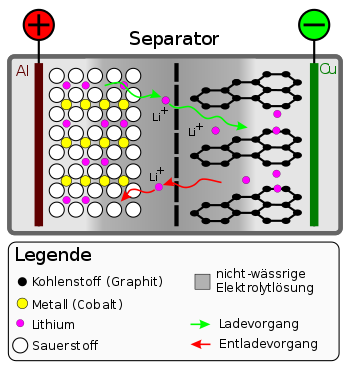
\includegraphics[scale=0.5]{figures/Akku/350px-Li-Ion-Zelle_(CoO2-Carbon,_Schema).svg.png}
		\caption{Grundaufbau einer Lithium-Ionen Zelle}
	\end{center}
\end{figure}
\newpage

\subsubsection{Lagerung und Sicherheithinweise}
Auch wenn Lithium nur als Li-Verbindungen in Lithium-Ionen Akkumualtoren vorhanden sind, sind die Komponenten eines solchen Akkus extrem leicht entzündbar, da Lithium ein hochreaktives Metall ist. Beim Überladen sind Ausgleichsreaktionen (z.B. die Zersetzung von Wasser), bei Lithium-Ionen Akkus nicht möglich, wie bei anderen Akkumualtoren dies der Fall ist. Schutzschaltungen die intern verbaut sein sollten, müssen eine solche Verpufferung verhindern. Anderfalls wird sonst die Funktionsfähigkeit des Akkus zerstört und er wird unbrauchbar. 
Jedoch kann es nicht nur zu inneren Beschädigungen kommen. Im Falle von inneren Kurzschlüssen, kann es passieren, dass mechanische Beschädigungen entstehen. Der hohe Kurzschlussstrom lässt zum Beispiel das Gehäuse schmelzen oder sogar in Flammen aufgehen. Es kann auch passieren, dass man den Defekt nicht unmittelbar erkennen kann. Doch kurze Zeit später kann es bereits zum Ausbruch eines Feuers kommen.

\textbf{Lagerung:}

Im Idealfall, sollten Lithium Ionen Akkus bei einem Ladezustand zwischen 40 - 60 Prozent kühl aufbewahrt und gelagert werden.


\textbf{Sicherheitshinweise:}

\begin{itemize}
	\item{Es ist wichtig, dass Lithium-Ionen Akkus nur mit passenden Ladegeräten aufgeladen werden. Schnell-Ladegeräte für Lithium Akkumulatoren können beispielweise eingesetzt werden. Man muss darauf achten, dass sie immer unter Aufsicht und möglichst nicht in der Nähe von brennbaren Materialien benutzt werden.} \medskip\\

	\item {Lithium-Ionen Akkus sind zwar hermetisch gekapselt, dennoch sollten sie unter keinen Umständen in Wasser getaucht werden. Besonders defekte und  vollgelade Lithium-Zellen reagieren meist heftig mit Wasser.}\medskip\\
	
	\item {Lithium-Ionen Akkumulatoren sind mechanisch sehr empfindlich. Durch einen internen Kurzschluss und einem Kontakt mit Luft können sie sich schnell entzünden.}\medskip\\
	
	\item {Eine Lithium-Ionen Zelle die in Flammen steht, wenn möglich mit Sand und nicht mit Wasser löschen, da dies zu einer heftigen Reaktion führen kann.}\medskip\\
	
	\item {Lithium-Zellen sollten niemals über 4,2V geladen und nicht unter 2,5V pro Zelle entladen werden. Außerdem dürfen Zellen niemals kurzgeschlossen werden. Bei einem Ladvorgang ist auf eine gute Wärmeabfuhr zu achten (nicht in die Sonne legen).}\medskip\\
	
	\item {Mehrere Lithium-Zellen sollten nur dann gleichzeitig geladen werden, wenn eine Schutzschaltung vorhanden ist.}\medskip\\
	
	\item {Die Elektorlytflüssigkeit ist brennbar. Sollte aus einer Zelle Elektrolytflüssigkeit austreten, diese am besten sofort ordnungsgerecht entsorgen.}\medskip\\
	
	\item {Man sollte versuchen die Lithium-Zellen bei einer Restkapazität von 20 Prozent nachzuladen.}\medskip\\

\end{itemize}
\newpage

\subsubsection{Anwendungbereiche von Lithium-Ionen Akkumulatoren}
Lithium-Ionen Akkus versorgten anfangs hauptsächlich tragbare Geräte mit hohem Energiebedarf, für die herkömmliche Nickel-Cadmium- oder Nickel-Metallhydrid Akkus zu schwer oder zu groß waren, beispielsweise Mobiltelefone, Tablets, Digitalkameras, Camcorder, Notebooks, Handheld-Konsolen oder Taschenlampen. In der heutigen Zeit sind Lithium-Ionen Akkumulatoren fast in allen denkbaren Bereichen aufzufinden. In der Elektromobiliätsbranche dienen sie oftmals als Energiespeicher für Elektroautos, moderne elektronisch betriebene Rollstühle und auch für Hybridfahrzeuge. Auch im Modellbau haben sie schon früh Verwendung gefunden. Dadurch, dass Lithium Akkus ein deutlich geringeres Gewicht als andere Batteriearten aufweisen, sind sie in Verbindung mit bürstenlosen Gleichstrommotoren und den entsprechenden Reglern, gut als Antriebseinheit im Flugmodellbau geeignet. Scho seit Anfang des 21. Jahrhunderts, gibt es Lithium-Ionen Akkus auch in Elektrowerkzeugen wie zum Beispiel Akkuschraubern. Auch im Flugbetrieb haben diese Batterien Verwendung gefunden. In der Boeing 787 werden ebenfalls Lithium-Kobaltoxid-Akkus (LiCoO2) verwendet. Zum Großen Teil werden Lithium-Ionen-Batterie-Systeme auch in Batterie-Speicherkraftwerken und Solarbatterien eingesetzt.
\newpage


\subsection{Batteriemanagementsystem}
\label{Batteriemanagementsystem}
Batteriemanagementsysteme (BMS) sind elektronische Regelschaltungen, die Akkumulatoren oder Akkupacks auf Ladung und Entladung überwachen und ebenfalls regeln. Die Batteriekennwerte die man überwachen kann bzw. möchte, hängen oftmals von dem Projekt ab. Zu den häufigsten Batteriekennwerten gehören die Erkennung des Batterietyps, die Batteriespannung, die Spannung sowie die Temperatur einzelner Batteriezellen, die Akkukapazität, der Ladzusatnd, die Restbetriebszeit, die Stromentnahme und einige Kennwerte mehr. Die Hauptaufgabe von BMS-Systemen besteht darin, sicherzustellen, dass die Restenergie in einer Zelle optimal genutzt wird. Um keine Beschädigungen an Zellen zu bekommen, schützt das Batteriemanagementsystem die Batterien vor Tiefenentladung, vor Überspannung, vor zu schneller Ladung (begrenzen des Ladestroms) und ebenfalls vor einem zu hohen Entladestrom. Bei Akkupacks, d.h. Akkumulatoren mit mehreren Zellen, sorgt das Batteriemanagementsystem außerdem für ein sogenanntes Balancing, das sich darin ausdrückt, dass die verschiedenen Batteriezellen gleiche Ladezustände und Entladezustände haben.

\begin{figure}[H]
	\begin{center}
		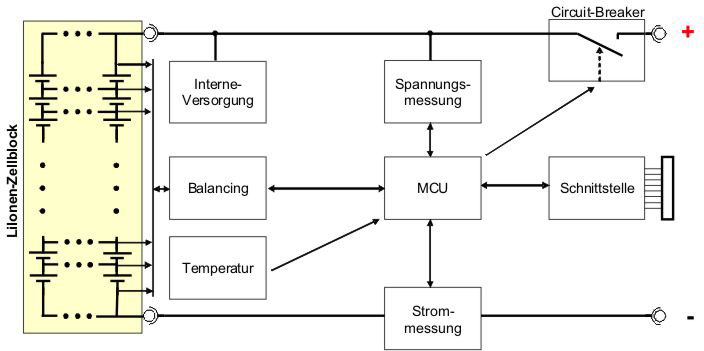
\includegraphics[scale=0.5]{figures/Akku/bms-1schaltunggrund.jpg}
		\caption{Grundschaltung eines Batteriemanagementsystems}
	\end{center}
\end{figure}

Grundsätzlich setzt sich ein vollständiges Batteriemanagementsystem aus folgenden Komponenten zusammen:
\begin{itemize}
	\item \textbf{Cell Supervising Circuit(CSC):} \medskip\\
	Die Aufgabe des CSC besteht darin die Zellen auf Spannung und 			Temperatur zu überwachen.

	\item \textbf{Kontrolleinheit:}\medskip\\
	Die Kontrolleinheit berechnet die State of Charge (SOC), die State 	of Health (SOH) und überprüft auch die Funktionalität der 				Batterien (State of Function). Außerdem wird von der 					Kontrolleinheit auch der Ladeausgleich gesteuert und kommuniziert 		über eine Serielle Schnittstelle mit einem Prozessor. 

	\item \textbf{Circuit Breaker:}\medskip\\
	Der Circuit Breaker trennt im Fehlerfall die Batterie von der 		Last. Dies erfolgt mithilfe eines HS-Kontaktors.
	
	\item \textbf{Strommessvorrichtung:}\medskip\\
	Diese Komponente ist für die Messung des Stromes zuständig.
	
	\item \textbf{Temperaturüberwachung:}\medskip\\
	Diese Komponente überprüft, ob sich die Batterien oder die 				Akkupacks in einem zulässigen Temperaturbereich befinden.
\end{itemize}
\newpage

\subsubsection{Komponenten eines BMS}

\textbf{Cell Supervising Circuit (CSC):}
Die erste Komponente eines Batteriemanagementsystem ist für die Spannungs- und Temperaturüberwachung der einzelnen Zellen zuständig und wird als Cell Supervising Circuit (CSC) bezeichnet. Ein Akkusystem besteht immer aus mindestens 2 einzelnen Zellen, oftmals jedoch aus mehreren. Deswegen ist die Spannungs- und Temperaturüberwachung jeder einzelnen Zelle nicht möglich. Es kommt  durchaus vor, dass mehrere einzelne Zellen zu sogenannten Akkupacks zusammengeschraubt oder zusammengeschweißt werden. Man hat dann wiederrum die Möglichkeit, jedes Akkupack für sich mithilfe eines CSC zu überwachen.

\textbf{Kontrolleinheit:}
Die nächste Komponente wird auch als Kontrolleinheit bezeichnet. Die Aufgabe dieser Komponente liegt darin, die SOC (State of Charge) und auch die SOH (State of Health) zu berechnen. Außerdem steuert die Kontrolleinheit auch den Ladeausgleich der einzelnen Zellen oder der Akkupacks. Diese Komponente übernimmt auch die Kommunikation des Batteriemanagementsystems mit anderen angeschlossenen Einheiten. Diese Kommunikation erfolgt über eine serielle Schnittstelle wie den I2C-Bus oder dem CAN-Bus. Die Werte (SOC und SOH) und auch die SOF (State of Function) werden dann an einen Prozessor übermittel auf dem die BMS-Software läuft und außerdem der SOC-Algorithmus implementiert ist. Die Kontrolleinheit ist fähig sich selbst in einen Ruhezustand zu versetzen um den eigenen Stromverbauch um ein Minimum zu reduzieren.

\begin{itemize}
	\item \textbf{State of Health (SOH):} \medskip\\
	Beschreibt den aktuellen Alterungszustand der Batterie. Ein Kriterium dafür ist, welche Ladungsmengen die Zellen noch aufnehmen. Je älter die Akkumulatoren werden, desto weniger Aufnahmevermögen haben sie.

\item \textbf{State of Charge (SOC):} \medskip\\
	Beschreibt den momentanen Ladezustand der Batterie. Außerdem gibt er Auskunft darüber, wie viel beziehungsweise wie lange die Batterie noch Energie bereitstellt. Beim Aufladen der Akkus gibt es an, wie viel Energie er noch aufnehmen kann.

\item \textbf{State of Function (SOF):} \medskip\\
	Gibt die Funktionalität der Batterie an. State of Function beschreibt die Leistungsfähigkeit der Batterie. Also wie viel kW der Energiespeicher dem Motor zum Beispiel bereitstellen kann. Die Leistungsfähigkeit lässt mit zunehmendem Batteriealter nach.
\end{itemize}

\textbf{Circuit-Breaker:}
Tritt ein Fehler bei einer einzelnen Zelle oder auch einem ganzen Akkupack auf, wird diese Batterie mithilfe eines HS-Kontaktors (Circuit-Breaker) von der Last getrennt. Dies schützt den Akkumulator. Dieser Kontaktor übernimmt außerdem noch die Trennung eines Akkumulatoren im Ruhezustand. Fehler die durch Trennen der Last beseitig werden können sind zum Beispiel Kurzschlüsse oder auch Übertemperatur. Für den Kurzschlussfall sind meisten auch noch Schmelzsicherungen (eine Art Sollbruchstelle im Stromkreis; die Wärmewirkung des Stromes wird ausgenutzt) verbaut die verhindern, dass Leitungen oder auch das Gehäuse in Flammen aufgehen.

\textbf{Strommessvorrichtung:}
Diese Komponete ist wie der Name schon beschreibt, für die Messung des Stromes zuständig. Oftmals werden dazu zwei voneinander unabhängige Systeme verwendet. Um den Strom messen zu können, wird ein Messsensor verwendet. Dies ist meist ein einfacher Widerstand. Bei der zweiten Methode wird der Strom über das elektromagnetische Feld gemessen.

\textbf{Temperaturüberwachung:}
Die letzte Komponente, die benötigt wird, um das Batteriemanagementsystem zu vervollständigen, ist für den Temperaturausgleich zuständig. Das heißt, es wird überwacht ob sich der Akkumulator in einem zulässigen Temperaturbereich findet. Sollte das nicht der Fall sein, können innere sowie auch äußere Schäden an der Batterie entstehen. Außerdem wirkt sich die Temperatur auf die Lebensdauer der Akkus auf.
\newpage

\subsubsection{Battery-Balancing}
\label{Battery-Balancing}
Der Ausdruck Balancing bezogen auf Akkumulatoren bedeutet so viel wie Ladeausgleich. Ohne Battery-Balancing bestimmt in einem Mehrzellen-Akku immer die schwächste Zelle darüber, welche Kapazität oder Spannung das Gesamtsystem aufweist. Das ergibt sich daraus, da sich jede Zelle minimal von einer anderen Zelle, durch ihre chemischen Struktur, unterscheidet. Einzelne Batteriezellen können auch unterschiedlich altern und deswegen kann man nie sicherstellen, dass jede Zelle exakt die identische Kapazität aufweist. Manche Zellen laden etwas schneller oder langsamer als andere. Wiederrum andere Batterien entladen sich etwas zügiger oder eben auch langsamer. In der Regel gibt es zwei verschiedene Arten von Battery-Balancing.
\begin{itemize}
\item \textbf{Passives Battery-Balancing} \medskip\\
\item \textbf{Aktives Battery-Balancing} \medskip\\
\end{itemize}


\textbf{Akkupacks:}

Muss noch zitiert werden: Cluster oder Akkupacks bestehen zur Erhöhung der Nennspannung in der Regel aus mehreren in Reihe geschalteten Einzelzellen oder Zellblöcken. Fertigungs- und alterungsbedingt gibt es hierbei Schwankungen in der Kapazität, im Innenwiderstand und weiteren Parametern dieser Zellen. Die schwächste Zelle ist dabei bestimmend, wie viel geladen oder entladen werden darf. Im praktischen Einsatz von mehrzelligen in Reihe verschalteten Akkus führt dieser Umstand dazu, dass die Zellen in Reihe unterschiedlich geladen und entladen werden.

Es kommt dann im Verbund zu kritischer Tiefentladung oder bei der Ladung zu einer Überladung und Überschreiten der Ladeschlussspannung einzelner Zellen. Je nach Akkutyp kann es dabei zu einer irreversiblen Schädigung einzelner Zellen kommen. Die Folge: das gesamte Akkupack verliert an Kapazität. (Ende des Zitates)
Um das zu verhindern, spielen im Batteriemanagementsystem die Balancer eine wichtige Rolle. Beim Battery-Balancing gibt es zwei verschiedene Arten. 
\begin{itemize}
\item \textbf{Passives Battery-Balancing} \medskip\\
\item \textbf{Aktives Battery-Balancing} \medskip\\
\end{itemize}


\section{Synchronmaschine mit Dauermagneterregung}
\subsection{Auswertung der Antriebswelle (Encoder)}

\section{Curtis Controller}
\subsection{Allgemeines}
\subsection{Feldorientierte Regelung}

\section{Leonard-Umformer}
\subsection{Allgemeines}
\subsection{ }

\newpage

\section{PID-Regler}
\subsection{Einleitung}
Regelungen sind ein Bestandteil unseres Lebens und das nicht nur seit Erfindung der Dampfmaschine.

Allein schon der aufrechte Gang funktioniert nur mit Regelung. Dabei wirken die Sinne als Sensoren, das Gehirn als Regler und die Muskeln als Aktuatoren. Weitere Regelungen in unserem Körper sind z.B. die Konstanthaltung der Körpertemperatur, der Blutdruck, die Anpassung der Pupille auf Helligkeitsänderungen usw.

Der Begriff Regelung ist zu unterscheiden von dem im allgemeinen Sprachgebrauch oft synonym gebrauchten Begriff der Steuerung. Das Steuern ist ein rein vorwärts gerichteter Prozess ohne Rückkopplung. Die Ausgangsgröße wird dabei nicht überwacht und kann sich durch Störungen von außen verändern. Ein Beispiel ist die Steuerung eines Motors mit einer einstellbaren Spannung. Durch Laständerungen wird sich die Drehzahl des Motors ändern. Soll nun die Drehzahl konstant gehalten werden, bedarf es einer Rückkopplung um über die Spannung die Drehzahl anzupassen. Diese Rückkopplung ist das Kennzeichen einer Regelung.

Das Regeln ist ein Vorgang, bei dem die Ausgangsgröße, im Beispiel die Drehzahl, fortlaufend überwacht wird und bei Abweichung über die Stellgröße, im Beispiel die Spannung, korrigiert wird. Der sich dabei ergebende Wirkungsablauf findet in einem geschlossenen Kreis, dem Regelkreis, statt.
\vspace{5mm}

\subsection{Der Regelkreis}
Das Prinzip einer Regelung ist das fortlaufende: Messen – Vergleichen – Stellen
\\[5mm]

\begin{itemize}
	\item \textbf{Messen}
	\\[1mm] Die Regelgröße wird direkt oder mittels Sensoren gemessen.
	\medskip
	\item \textbf{Vergleichen}
	\\[1mm] Der Wert der Regelgröße wird mit dem Sollwert verglichen. Die Differenz ist die Regelabweichung.
	\medskip
	\item \textbf{Stellen}
	\\[1mm] Aus der Regelabweichung wird unter Berücksichtigung der dynamischen Eigenschaften der Regelstrecke die Stellgröße bestimmt.
\end{itemize}
\vspace{3mm}

Ein Regelkreis dient dazu, eine vorgegebene physikalische Größe, die Regelgröße, auf einen gewünschten Wert (Sollwert) zu bringen und dort zu halten, unabhängig von eventuell auftretenden Störungen. Um die Regelungsaufgabe zu erfüllen, muss der Augenblickswert der Regelgröße – der Istwert – gemessen und mit dem Sollwert verglichen werden. Bei auftretenden Abweichungen muss in geeigneter Art und Weise nachgestellt werden.

Um nun diese Aufgabe technisch zu lösen, gibt es die Regelungstechnik. Sie baut im wesentlichen auf die mathematische Beschreibung und Modellbildung des Systems Regelkreis. Zur Modellierung, Beschreibung und Simulation werden Blockschaltbilder mit diskreten Signalgliedern verwendet.

\newpage

Ein Regelkreis besteht entsprechend des vereinfachten Blockschaltbildes, wie es oft in der Regelungstechnik verwendet wird, aus den Hauptteilen Regler und Regelstrecke:
\\[5mm]

\begin{itemize}
	\item \textbf{Regler G$_R$}
	\\[1mm] Ist der Teil des Regelkreises, der unter Berücksichtigung der dynamischen Eigenschaften der Regelstrecke aus der Regelabweichung die Korrekturmaßnahmen zum Ausregeln ergreift.
	\medskip
	\item \textbf{Regelstrecke G$_S$}
	\\[1mm] Ist der Teil des Regelkreises, der vom Regler ausgeregelt werden soll.
	\medskip
	\item \textbf{Führungsgröße w (Sollwert)}
	\\[1mm] Vorgegebener Wert, auf dem die Regelgröße durch die Regelung gehalten werden soll. Sie ist eine von der Regelung nicht beeinflusste Größe und wird von außen zugeführt.
	\medskip
	\item \textbf{Regelgröße x (Istwert)}
	\\[1mm] Ist die Ausgangsgröße der Regelstrecke, die zum Zweck des Regelns erfasst und zum Vergleich rückgeführt wird. In vielen Fällen ist in der Rückführung noch eine Messeinrichtung (Sensor) gezeichnet, die den Istwert erfasst, hier der Einfachheit halber weggelassen.
	\medskip
	\item \textbf{Regelabweichung e}
	\\[1mm] Differenz zwischen Führungsgröße und Regelgröße e = w – x, bildet die eigentliche Eingangsgröße des Reglers.
	\medskip
	\item \textbf{Stellgröße y}
	\\[1mm] Ausgangsgröße der Regeleinrichtung und zugleich Eingangsgröße der Strecke. Sie überträgt die steuernde Wirkung des Reglers auf die Strecke.
	\medskip
	\item \textbf{Störgröße z}
	\\[1mm] Eine von außen wirkende Größe, die eine Änderung des Istwertes der Regelgröße bewirkt und einen Regelvorgang auslöst.
\end{itemize}

\vspace{5mm}
\begin{figure}[H]
	\begin{center}
		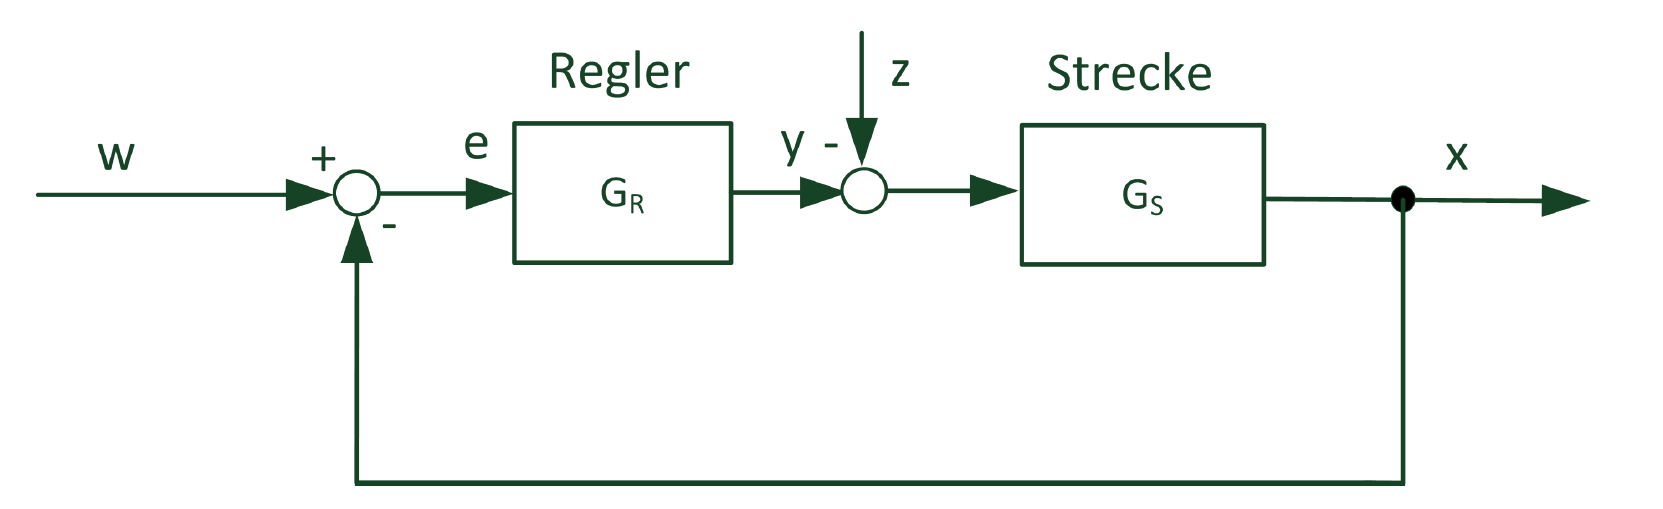
\includegraphics[width=\textwidth]{figures/antrieb/Regelkreis_Grundaufbau.png}
		\caption{Grundaufbau des allgemeinen Regelkreises}
	\end{center}
\end{figure}

\newpage

\subsection{Die Regelstrecke}
Die Regelstrecke stellt den zu regelnden Teil bzw. den zu regelnden Prozess dar und umfasst normalerweise eine Reihe von einzelnen Gliedern, welche das dynamische Verhalten der Regelstrecke beschreiben. Zur Unterteilung werden die Glieder entsprechend ihrem Zeitverhalten charakterisiert. Um das Zeitverhalten herauszufinden, legt man an den Eingang ein Testsignal an und zeichnet die Antwort auf. Im einfachsten Fall wird der Eingang mit einer sprunghaften Änderung beaufschlagt. Die Antwort auf die sprunghafte Änderung der Eingangsgröße wird Sprungantwort genannt und gibt Aufschluss über die Art der Regelstrecke und kann eventuell bereits genutzt werden, um die Parameter der Regelstrecke zu bestimmen.

Für den Aufbau eines gut funktionierenden Regelkreises und die Auslegung von Reglern ist es eine Voraussetzung zu wissen, wie die Regelstrecke reagiert. Ohne ein genaues Wissen um das dynamische Verhalten der Regelstrecke ist es nicht möglich geeignete Regler auszuwählen und diese zu parametrieren. Die einzelnen Eigenschaften der Glieder zu beschreiben würde aber den Rahmen sprengen.

\subsection{Der Regler}
Der Regler hat die Aufgabe, die Regelgröße zu messen, sie mit dem Sollwert zu vergleichen und bei Abweichungen die Stellgröße so zu verändern, dass Soll- und Istwert der Regelgröße wieder übereinstimmen bzw. die Differenz minimal wird.

Die Wahl eines bestimmten Reglertyps richtet sich nach dem geforderten Zeitverhalten und der geforderten Regelgenauigkeit der Regelstrecke. Nachfolgend finden Sie eine kurze Beschreibung der wichtigsten klassischen Reglertypen: 
\\[5mm]
\textbf{P-Regler}\\[1mm]
Der proportionalwirkende Regler multipliziert die Regelabweichung mit seinem Verstärkungsfaktor Kp und gibt das Ergebnis unverzögert weiter. Der P-geregelte Kreis ist einfach und mittelschnell im Vergleich zu anderen Regelungen. Das Problem ist die bleibende Regelabweichung!

Reglergleichung: \hspace{5mm} $y(t) = K_P \cdot e(t)$ \hspace{5mm} bzw. \hspace{5mm} G$_R$ = K$_P$
\\[5mm]

\textbf{I-Regler}\\[1mm]
Der integralwirkende Regler summiert die Regelabweichung über der Zeit auf und multipliziert die Summe (d.h. das Integral) mit dem Faktor Ki. Je länger eine Regelabweichung ansteht, desto größer wird die Stellgröße des I-Reglers. Der I-geregelte Kreis ist langsam im Vergleich zu anderen Regelungen. Er hat aber den Vorteil, dass die Abweichung vollständig eliminiert wird.

Reglergleichung: \hspace{5mm} $y(t) = K_I \cdot \int\limits_{0}^{t} e(t) \,dt$ \hspace{5mm} bzw. \hspace{5mm} $G_R = \dfrac{K_I}{s}$

\newpage

\textbf{PD-Regler}\\[1mm]
Der proportional-differential wirkende Regler kombiniert den P-Regler mit einem D-Anteil (einen D-Regler gibts es nicht). Der D-Anteil bewertet die Änderung einer Regelabweichung, er differenziert und berechnet so deren Änderungsgeschwindigkeit. Diese wird mit dem Faktor Kd multipliziert und zum P-Anteil hinzuaddiert. Der PD-Regler reagiert damit schon auf Ankündigungen von Veränderungen, das bewirkt sozusagen ein Vorhalten beim Regeln.

Der PD-geregelte Kreis ist sehr schnell im Vergleich zu anderen Regelungen, und manche Regelkreise (solche mit zweifacher Integration) sind ohne D-Anteil überhaupt nicht stabilisierbar. Das Problem des P-Reglers, die bleibende Regelabweichung, ist beim PD-Regler allerdings weiterhin vorhanden!

Ein Nachteil aller Regler mit D-Anteil kann die Unruhe im Kreis sein. Ist das Sensorsignal verrauscht, so wird dieses Rauschen durch das Differenzieren weiter verstärkt und wieder in den Kreis hineingegeben. Dadurch wird der Aktuator stärker belastet. Solche Probleme können aber durch Anpassung der Regelparameter oder mit dem Hinzufügen eines Filters behoben werden.

Reglergleichung: \hspace{5mm} $y(t) = K_P \cdot e(t) + K_D \cdot \dfrac{de(t)}{dt}$\hspace{5mm} bzw. \hspace{5mm} $G_R = K_P + K_D \cdot s$
\\[5mm]

\textbf{PID-Regler}\\[1mm]
Der PID Regler vereinigt die guten Eigenschaften der anderen Regler. Der PID-geregelte Kreis ist genau und sehr schnell. In den meisten Anwendungen kommt deshalb der PID-Regler zum Einsatz. Vorab sollte man jedoch überprüfen, ob ein einfacherer bzw. billigerer Regler für die Realisierung der gewünschten Anwendung ebenfalls ausreicht. 

Reglerleichung: \hspace{3mm} $y(t) = K_P \cdot e(t) + K_I \cdot \int\limits_{0}^{t} e(t) \,dt + K_D \cdot \dfrac{de(t)}{dt}$ \hspace{3mm} bzw. \hspace{3mm} $G_R = K_P + \dfrac{K_I}{s} + K_D \cdot s$

\begin{figure}[H]
	\begin{center}
		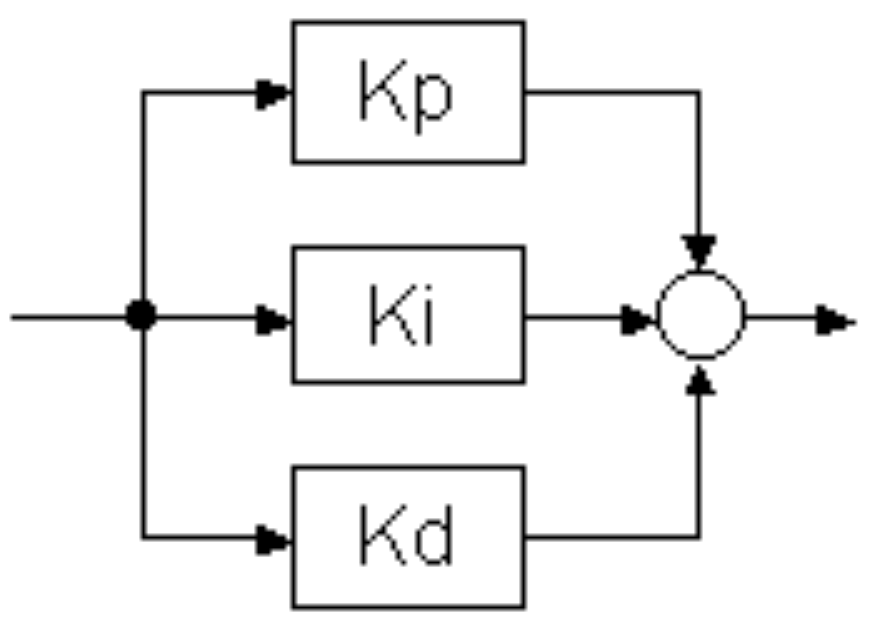
\includegraphics[scale=0.15]{figures/antrieb/PID_Regler.png}
		\caption{Zusammensetzung des PID-Reglers}
	\end{center}
\end{figure}

Hier ist für ein besseres Verständnis jeweils eine Sprungantwort der unterschiedlichen klassischen Reglertypen dargestellt:
 
\begin{figure}[H]
	\begin{center}
		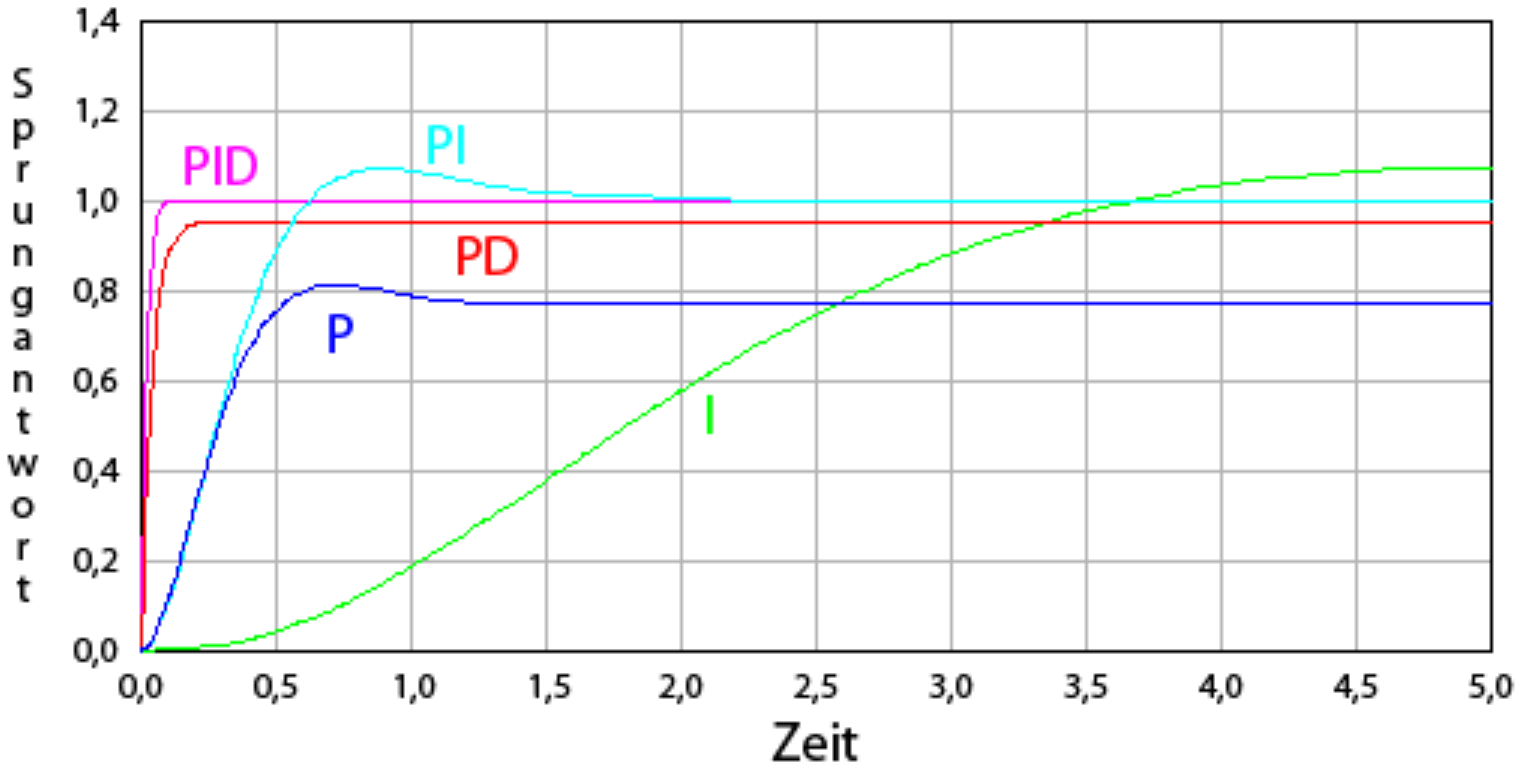
\includegraphics[scale=0.3]{figures/antrieb/Reglertypen.png}
		\caption{Vergleich der verschiedenen Reglertypen}
	\end{center}
\end{figure}
%https://rn-wissen.de/wiki/index.php/Regelungstechnik
%http://3digi.wikidot.com/allgemeines-zu-pid-reglern
%AUT5
\newpage

%%%%%%%%%%%%%%%%%%% HCIS

\section{Steuereinheiten}
\section{Bussysteme}
